\documentclass{article}
\usepackage{graphicx}
\usepackage{listings}
\usepackage{color}


\begin{document}

\title{Draw Forestogram in with rgl package}
\maketitle

\begin{abstract}
The abstract text goes here.
\end{abstract}

\section{Introduction}
%How is the forrestogramme build. 



\begin{figure}[h]

\[
Merge =  \left(\begin{array}{cc}
-1 & -2 \\
-1 & -2 \\
 1 & -3 \\
 2 & -4 \\ 
 1 & -3 
\end{array} \right)
%
Height = \left( \begin{array}{c}
1 \\
1.3 \\
4 \\
7 \\
10 
\end{array} \right)
%
Rowcol = \left( \begin{array}{c}
r \\
c \\
c \\
c \\
r 
\end{array} \right)
\]  
\end{figure}

\begin{figure}[h]
\centering 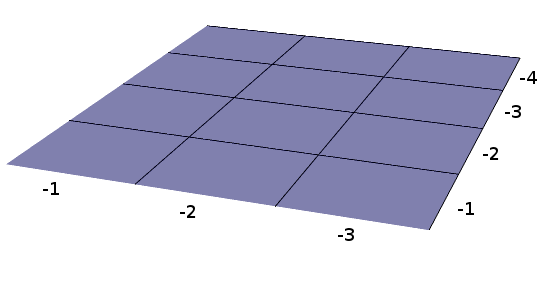
\includegraphics[scale=0.3]{base}
\end{figure}

\clearpage
\section{Step by step construction}



\raggedright\subsection{Step 1}
\[
Merge =  \left(\begin{array}{cc}
-1 & -2 \\
\end{array} \right)
%
Height = \left( \begin{array}{c}
1 \\
\end{array} \right)
%
Rowcol = \left( \begin{array}{c}
r \\
\end{array} \right)
\]  


%\centering 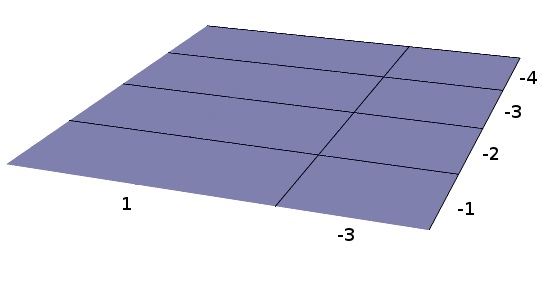
\includegraphics[scale=0.3]{base1}
\centering 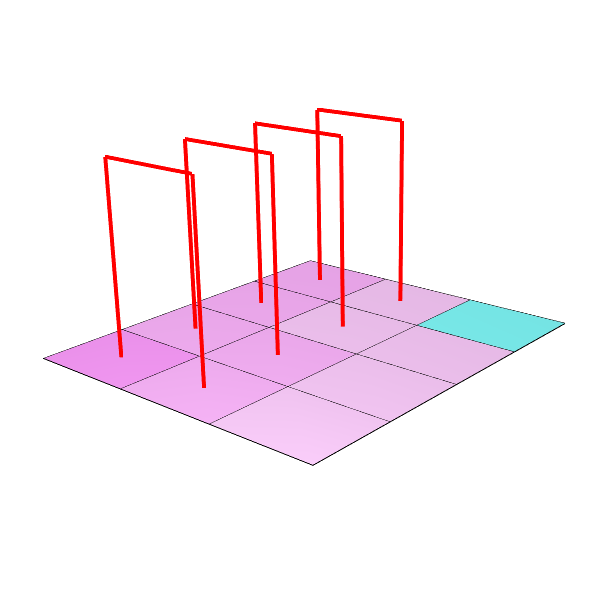
\includegraphics[scale=0.3]{Merge1}

\raggedright\subsection{Step 2}
\[
Merge =  \left(\begin{array}{cc}
-1 & -2 \\
\end{array} \right)
%
Height = \left( \begin{array}{c}
1.3 \\
\end{array} \right)
%
Rowcol = \left( \begin{array}{c}
c \\
\end{array} \right)
\]  

\centering 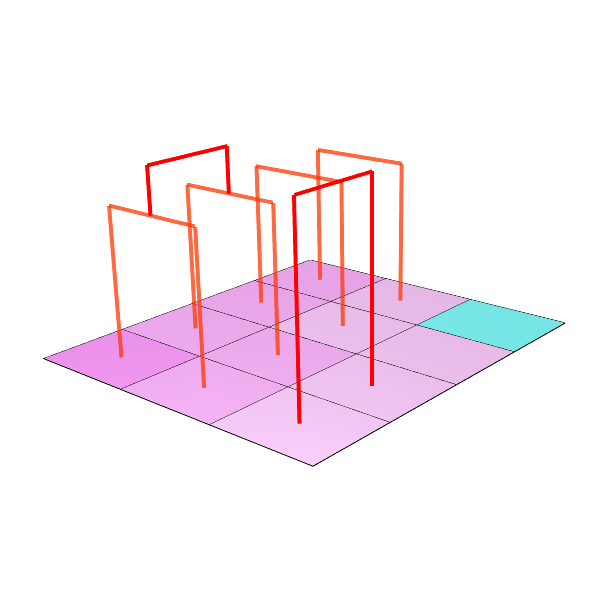
\includegraphics[scale=0.3]{Merge2}

\clearpage
%------------------------------------------------------------------------
\raggedright\subsection{Step 3}
\[
Merge =  \left(\begin{array}{cc}
1 & -3 \\
\end{array} \right)
%
Height = \left( \begin{array}{c}
4 \\
\end{array} \right)
%
Rowcol = \left( \begin{array}{c}
c \\
\end{array} \right)
\]  

\centering 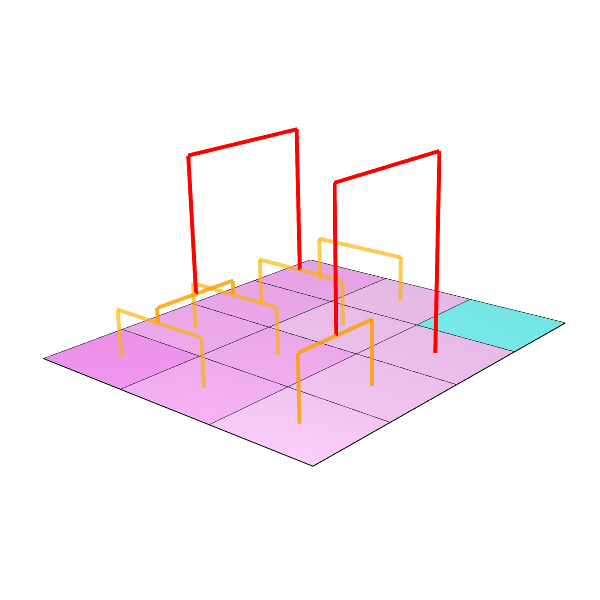
\includegraphics[scale=0.3]{Merge3}

%------------------------------------------------------------------------
\raggedright\subsection{Step 4}
\[
Merge =  \left(\begin{array}{cc}
2 & -4 \\
\end{array} \right)
%
Height = \left( \begin{array}{c}
7 \\
\end{array} \right)
%
Rowcol = \left( \begin{array}{c}
c \\
\end{array} \right)
\]  

\centering 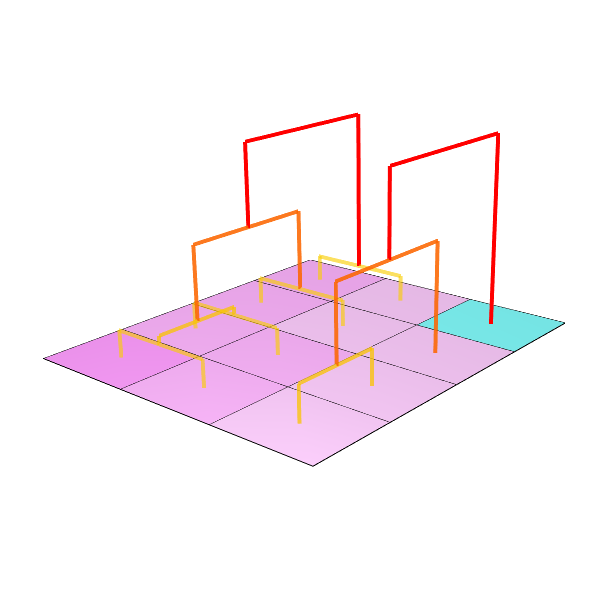
\includegraphics[scale=0.3]{Merge4}
\clearpage
%------------------------------------------------------------------------
\raggedright\subsection{Step 5}
\[
Merge =  \left(\begin{array}{cc}
1 & -3 \\
\end{array} \right)
%
Height = \left( \begin{array}{c}
10 \\
\end{array} \right)
%
Rowcol = \left( \begin{array}{c}
r \\
\end{array} \right)
\]  

\centering 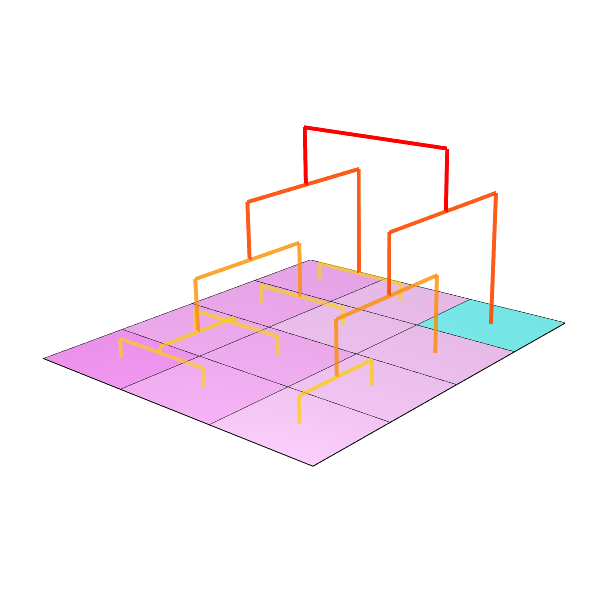
\includegraphics[scale=0.3]{Merge5}

\raggedright


\section{Implementation in R}

\lstset{ %
	language=R,
	numbers=left,
	frame=single,
	keywordstyle=\color[rgb]{0, 0, 0},
	commentstyle=\color[rgb]{0.5,0.5,0.5},
	stringstyle=\color[rgb]{0, 0, 0}
}
\begin{lstlisting}[]
library(rgl)
source('Function.R')

# Matrix size.
size = c(3, 4)

# Example tree drawing.
values =  c(-1, -2, -1, -2, 1, -3, 2, -4, 1, -3)
merges = MergeMatrix(size, values)
heights = c(1, 1.3, 4, 7, 10)
rowcols = c(0, 1, 1, 1, 0)

# Plot forestogramme.
Forestogramme(size, merges, heights, rowcols)
\end{lstlisting}
\section{Render forestogramme with rgl package}

\section{Conclusion}
Write your conclusion here.

\end{document}


